\documentclass[12pt, hyperref={unicode}]{beamer}
 
\usepackage[czech]{babel}
\usepackage[utf8]{inputenc}
\usepackage{graphicx}
\usepackage{algorithm}
\usepackage{algorithmic}
\usetheme{metropolis}


\graphicspath{{image/}} 

\title{Řadící algoritmy \\ Řazení výběrem}
\author{Pavel Yadlouski (xyadlo00)}
\institute{Vysoké učení technické v Brně \\  Fakulta informačních technologii}
\date{\today}

\begin{document}

\begin{frame}
	\titlepage
\end{frame}

\section{Řadící algoritmy}
\begin{frame}
	\frametitle{Definice problému}
	\begin{itemize}
		\item Na vstupu je posloupnost $S = (S_1,S_2,\ldots,S_n)$	
		\pause		
		\item Cílem je najít takovou posloupnost $S' = (S'_1,S'_2,\ldots,S'_n)$ pro kterou platí dvě základní kritéria
		\begin{enumerate}
			\item Tato posloupnost je seřazená: \\ $S'_1 \leq S'_2 \leq \ldots \leq S'_n$ 
			\item Poslopnost $S'$ je permutací původní poslopnosti $S$		
		\end{enumerate}
	\end{itemize}
		
\end{frame}

\begin{frame}
	\frametitle{Klasifikace algoritmů}
	\begin{itemize}
		\item \textit{vnitřní} řazení: \\ metody vycházejí z předpokladu, že všechna data se vejdou
do paměti.
		\pause
		\item \textit{vnější} řazení: \\ používáme tehdy, když objem dat je tak veliký, že nestačí
vnitřní paměť a musíme tedy využít i paměť vnější.
	\end{itemize}	
\end{frame}

\section{Řazení výběrem}
\begin{frame}
	\frametitle{Řazení výběrem (anglicky Selection sort)}
	\textbf{Řazení výběrem} je jednoduchý algoritmus uspořádávání s časovou
složitostí $O(N^2)$. Pro svou jednoduchou implementaci bývá často používán pro uspořádávání
malých množství dat.
\end{frame}

\begin{frame}
	\frametitle{Algoritmus řazení výběrem -- princip fungování }
	\begin{enumerate}
		\item Nastavíme $MIN$ na prvný index v posloupnosti $A$
			\pause		
		\item Najdeme prvek s nejmenší hodnotou
			\pause
		\item Zaměníme ho s prvkem na pozici $MIN$
			\pause
		\item Incrementujeme $MIN$ na další index
			\pause
		\item Zbytek posloupnosti se uspořádá opakováním kroků 2 až 4 pro zbylou neseřazenou část
	\end{enumerate}
\end{frame}

\begin{frame}
	\frametitle{Pseudokód}
	
	\begin{algorithmic}[1]
		\FOR {$i = 0$ to $N - 1$}
			\STATE $MIN = i$
			\FOR {$k = i + 1$ to $N$}
				\IF{$A[k] < A[MIN]$}
					\STATE $MIN = j$
				\ENDIF				
			\ENDFOR		
			\STATE swap $S[i] \Leftrightarrow A[MIN]$		
		\ENDFOR
	\end{algorithmic}
\end{frame}

\begin{frame}
	\frametitle{Průběh}
	\only<1>{
	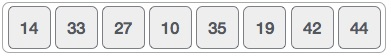
\includegraphics[scale=0.4]{image1} \\
	\vspace{0.5em}
	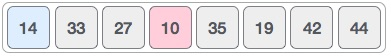
\includegraphics[scale=0.4]{image2} \\
	\vspace{0.5em}	
	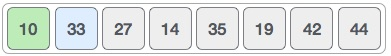
\includegraphics[scale=0.4]{image3} \\
	\vspace{0.5em}
	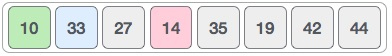
\includegraphics[scale=0.4]{image4}} 
	\only<2>{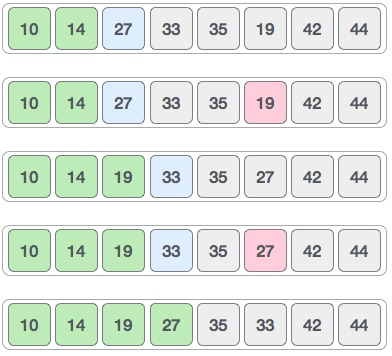
\includegraphics[scale=0.4]{image6}}
	\only<3>{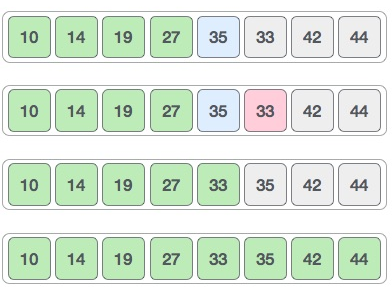
\includegraphics[scale=0.4]{image5}} 	
\end{frame}

\begin{frame}
	\frametitle{Použíte zdroje}
	\begin{itemize}
		\item Referenční zdroje \\
			\url {https://en.wikipedia.org/wiki/Sorting_algorithm}		
		\item Obrázky \\
			\url{https://www.tutorialspoint.com/data_structures_algorithms/selection_sort_algorithm.htm}
	\end{itemize}
\end{frame}
\end{document}


